



\subsection{Autenticazione}


Poiché la modalità di autenticazione rappresenta un elemento cruciale per l’esperienza dell’utente, 
in quanto deve assicurare un accesso sicuro all’applicazione mantenendone la semplicità, la facilità del processo autenticazione deve essere garantita.
Offrire agli utenti la possibilità di autenticarsi tramite il proprio authentication provider di fiducia migliora sicuramente l’usabilità e l’apprezzamento degli utenti, 
ma è altrettanto essenziale consentire la possibilità di creare account dedicati esclusivamente all’applicazione.
Di conseguenza, il sistema di gestione degli accessi deve supportare sia la registrazione e la gestione autonoma degli account specifici per il servizio, 
sia fornire l'integrazione con provider di autenticazione esterni.\\
\\
Per lo scopo, Azure fornisce Microsoft Entra ID, parte della suite di servizi di autenticazione e autorizzazione Microsoft Entra. 
Sebbene teoricamente in grado di soddisfare i requisiti sopra indicati, 
la complessità della documentazione e le difficoltà riscontrate nell’integrazione con il servizio dell’applicativo
 hanno portato a valutare soluzioni alternative negli ambienti cloud.\\
\\
La scelta è ricaduta su Firebase Authentication, che garantisce sia la possibilità di creare account dedicati che di collegarsi attraverso altri authentication providers. 
Inoltre, la piattaforma presenta un’interfaccia chiara e offre servizi di integrazione di facile utilizzo sia tramite Flutter che tramite C\#.
Dal punto di vista economico, il servizio risulta vantaggioso, essendo gratuito fino ai cinquantamila utenti mensili attivi.\\
\\
Uno dei requisiti fondamentali del progetto prevede che ogni account sia associato in modo univoco a un singolo utente. 
Durante la fase di creazione del profilo, tuttavia, l’account viene inizialmente registrato nel database gestito da Firebase. 
Pertanto, al primo accesso, il server, dopo aver verificato l’autenticità della richiesta, provvede a creare una copia dell’account, 
generando poi il relativo nuovo oggetto utente e il primo profilo associato.\\
\clearpage
\begin{figure}[h!]
    \centering
    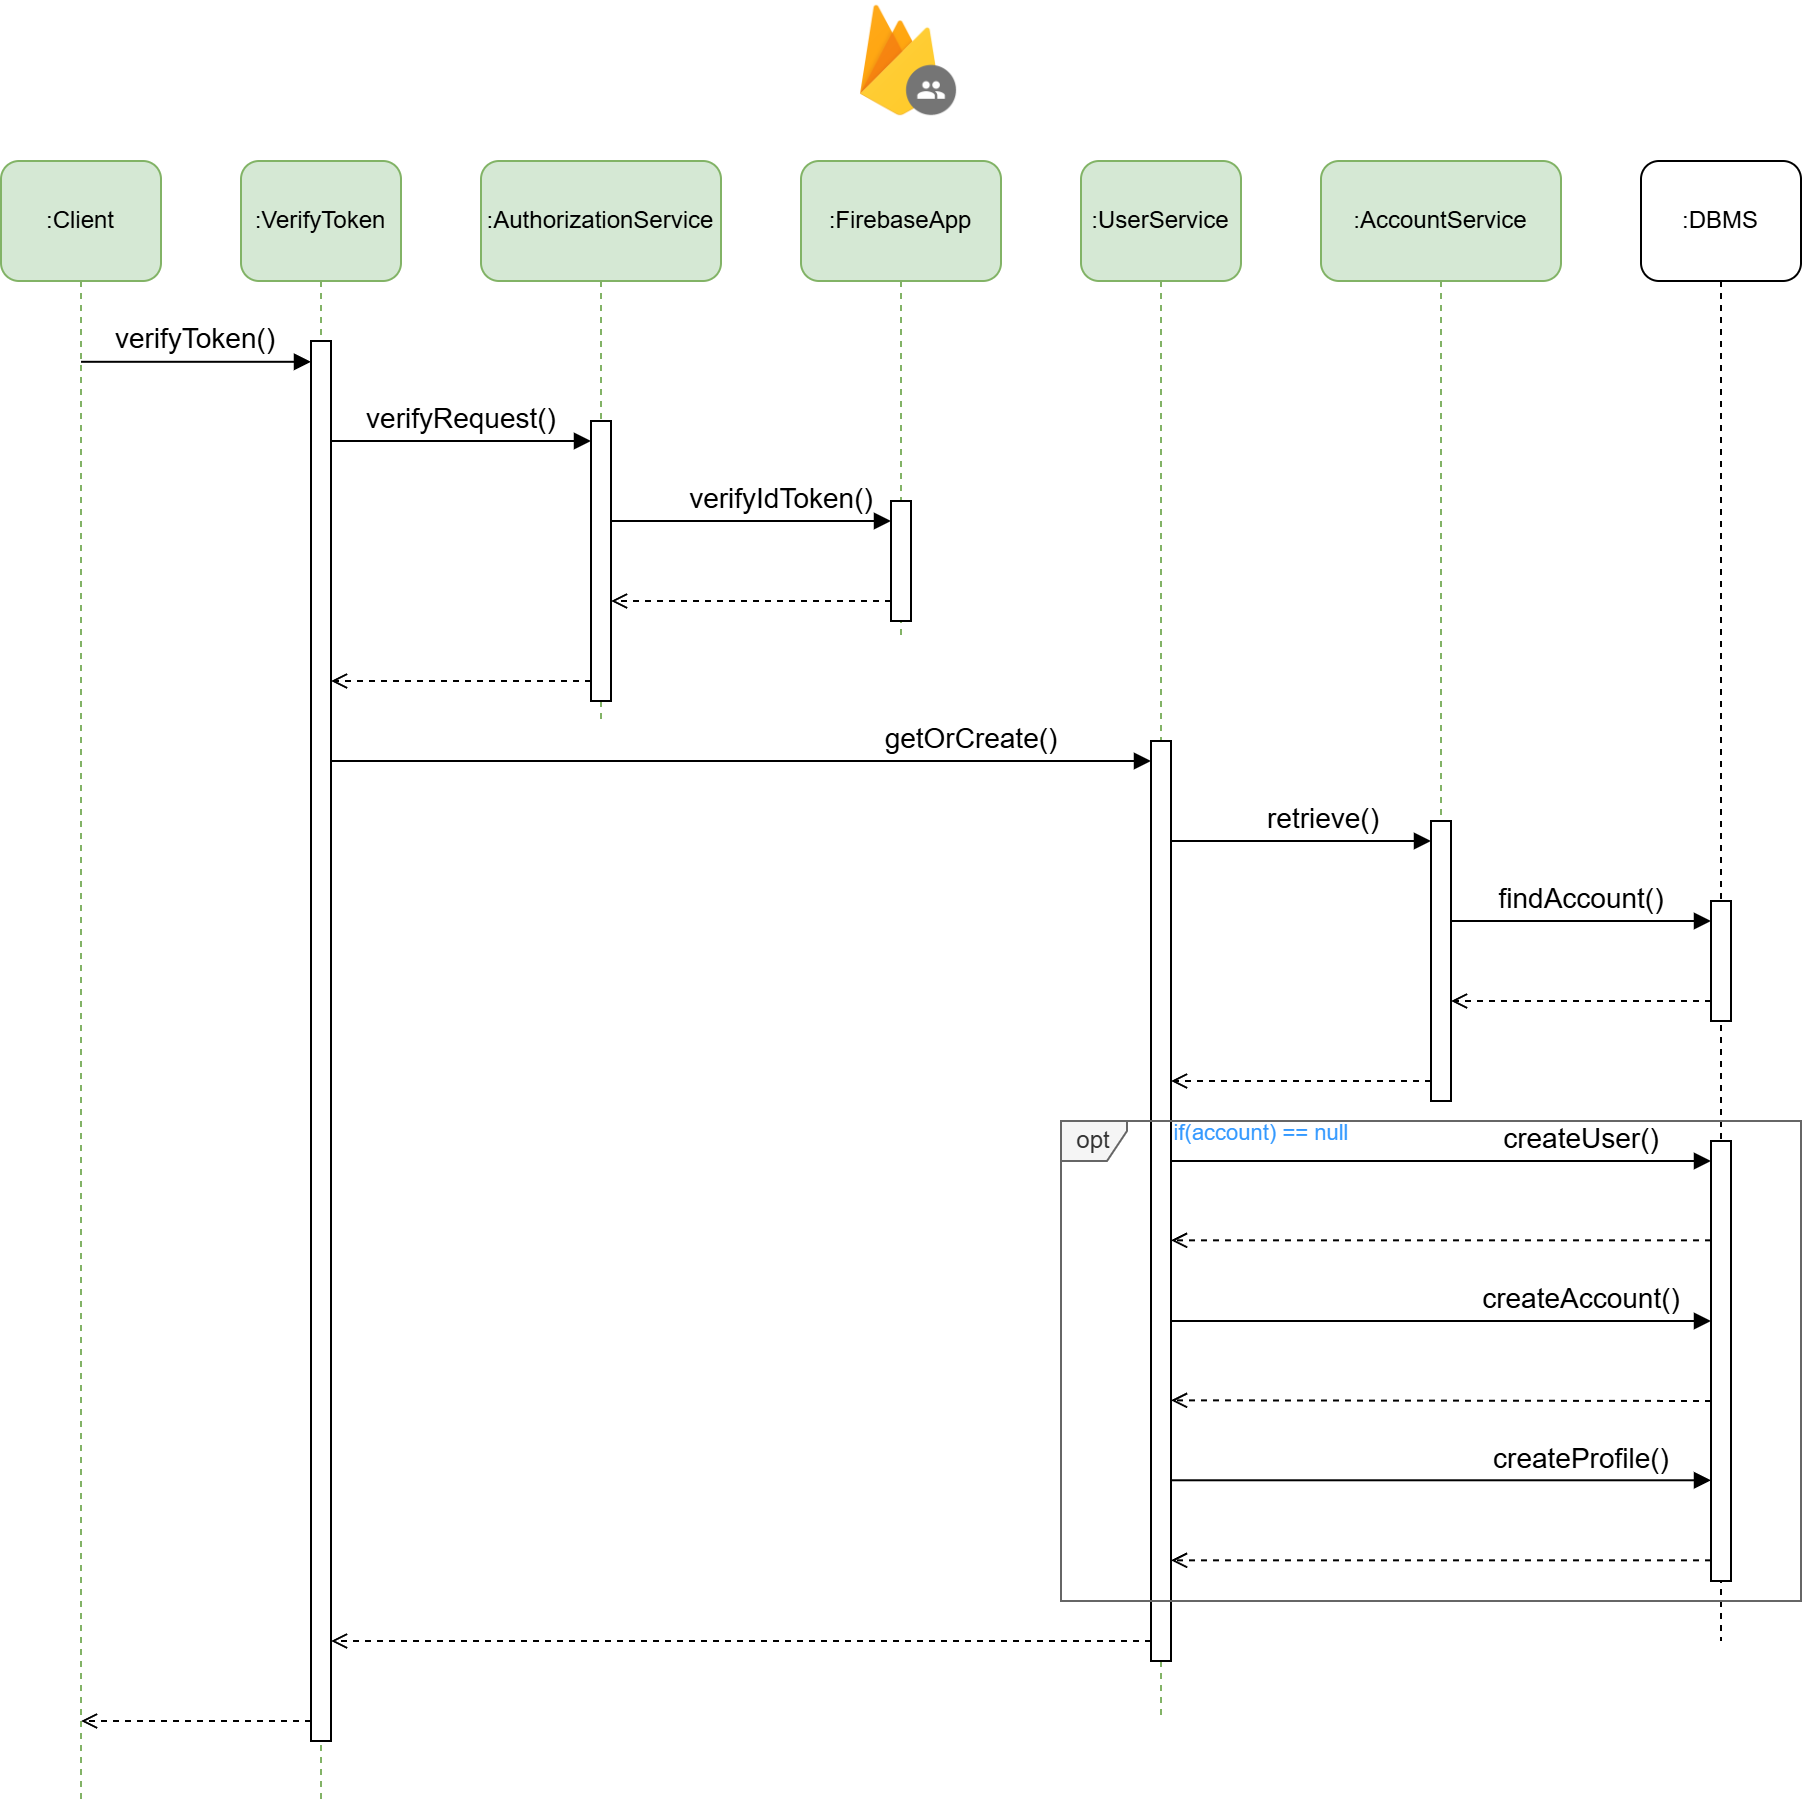
\includegraphics[width=\textwidth]{IIVerifyToken2.png}
    \caption{Diagramma di sequenza per la creazione di un account}
\end{figure}
Per garantire un processo di autenticazione sicuro ed efficiente, a ogni richiesta che richiede identificazione, 
il dispositivo utente aggiunge anche il token di autenticazione, salvato durante il primo accesso e la verifica iniziale. 
Il server verifica quindi la validità del token prima di procedere con l'esecuzione della richiesta.

\clearpage
\subsection{La sicurezza}

Il collegamento tra i vari componenti all’interno dell’ambiente Azure richiede l’utilizzo di chiavi e stringhe di connessione. 
Il salvataggio di tutte le chiavi sensibili è stato affidato al servizio Azure Key Vault,
 un server che permette la centralizzazione dei dati, cifrando il contenuto e garantendo un controllo maggiore sul loro utilizzo. 
Quando necessario i servizi, in particolare le Azure Functions, contatteranno il Key Vault per l’ottenimento delle chiavi necessarie, 
riducendo il rischio di un’intercettazione data magari da un errore durante lo sviluppo.\\
\\
Le comunicazioni tra i vari componenti devono avvenire in sicurezza, garantendo autenticità e confidenzialità. 
Per questo motivo tutte le comunicazioni tra dispositivi client e i vari servizi utilizzano la tecnologia TLS, che permette di cifrare i messaggi grazie ad uno standard collaudato. 
In particolare, le comunicazioni tra i client e Azure Functions, così come con Firebase Authentication e il server per la persistenza delle immagini, 
avvengono tramite protocollo HTTPS, mentre le comunicazioni con il server per gli aggiornamenti in tempo reale usano il protocollo WSS.\\
\\
L’accesso al database è ristretto alle sole risorse Azure, garantendo l’isolamento dall’esterno, che comprometterebbe altrimenti l’affidabilità dei dati.\\
\\
Infine, l’identificativo di ogni elemento del dominio è nascosto all’utente tramite la creazione di codici hash univoci 
che permettono comunque l’identificazione dell’oggetto senza rivelare ulteriori informazioni. 
In particolare, il caricamento delle immagini avviene grazie ad un link univoco dato dalla combinazione degli identificativi dell’evento e dell’immagine. 
Utilizzando i codici di hash diventa molto complicato il ritrovamento delle immagini senza essere a conoscenza dei codici, 
che non avendo natura incrementale ma distribuita rende indovinare un link valido.

\mycomment{
TODO Dos e limite alle dimensioni delle richieste
}
\clearpage
\subsection{Monitoraggio}

Il monitoraggio del sistema è attuato in due modalità: tramite salvataggio dei log e controllo delle prestazioni del sistema.\\
\\

Relativamente a Firebase Authentication vengono forniti con il servizio sia le interfacce
per il controllo delle prestazioni che la gestione dei log. Non è quindi richiesta alcuna ulteriore azione.\\
\\
Per monitorare le Azure Functions sarà invece necessario collegare Azure Application Insights, servizio che provvede a controllare il funzionamento e la risposta del servizio. 
Una volta unito il servizio, infatti, Azure Application Insight permette la presentazione e l'analisi di numerose metriche, quali il tempo di risposta e il consumo di risorse. 
Consente inoltre di testare la risposta dell’applicativo simulando diversi scenari e riassumendo il loro comportamento.\\
\\
La creazione dei log è invece delegata al programmatore, in quanto è necessario integrarli nel codice. 
Nel momento della creazione, ogni funzione riceve, tramite dependency injection, un servizio Logger che permette la creazione e il salvataggio dei log. 
Tali log saranno poi consultabili e analizzabili tramite l’interfaccia fornita da Azure Application Insight.\\
\\
\clearpage